\section{La dinámica analítica para el caso $\mcU=\textsc{SWAP}$}
En esta sección se desarrollan resultados analíticos para una evolución unitaria subyacente descrita por el operador \textsc{SWAP}.

\subsection{Evolución de $t=0$ a $t=1$}

Utilizando la expresión (\ref{eq:MaxEntSeparable}), se puede pasar tanto a $\varrho_{max}(0)$ como a $\varrho_{max}(1)$ a través de la aplicación de grano grueso. El resultado $\CG{\varrho_{max}(0)}$ corresponde al estado grueso inicial, pero en términos de $\lambda$. Así:
\begin{equation}
\rho(0)=\frac{1}{2}[\Id+(\hat{r}_{\rho}\cdot\vec{\sigma})(p\tanh{\lambda p}+(1-p)\tanh{\lambda (1-p)})],
\end{equation}
\begin{equation}
\rho(t=1)=\frac{1}{2}[\Id+(\hat{r}_{\rho}\cdot\vec{\sigma})((1-p)\tanh{\lambda p}+p\tanh{\lambda (1-p)})].
\end{equation}
Vemos que ambos estados tienen la misma orientación pero pureza distinta. Esto significa que el efecto del \textsc{SWAP} subyacente sobre la esfera de Bloch es comprimir al estado efectivo inicial con un coeficiente $\kappa_{1}$ tal que
\begin{equation}\label{eq:SWAPFactor}
  \kappa_{1}=\frac{r_{\rho(1)}}{r_{\rho(0)}}=\frac{(1-p)\tanh{\lambda p}+p\tanh{\lambda (1-p)}}{
    p\tanh{\lambda p}+(1-p)\tanh{\lambda (1-p)}}
\end{equation}
Claro está, el factor de compresión depende del multiplicador de Lagrange, que a su vez es una función de la pureza del estado inicial. La figura \ref{fig:SWAPFactor2D} muestra dicha dependencia. Si la dependencia del factor de compresión en el estado efectivo inicial se denota por un superíndice, la dinámica efectiva puede escribirse como
\begin{equation}\label{eq:EffectiveSWAP1}
  \boxed{\frac{1}{2}(\Id+\vec{r}_{\rho}\cdot\vec{\sigma}) \xrightarrow{S} \frac{1}{2}(\Id+\kappa_{1}^{\rho}\vec{r}_{\rho}\cdot\vec{\sigma})}
\end{equation}
De las ecuaciónes (\ref{eq:SWAPFactor}) y (\ref{eq:EffectiveSWAP1}) distinguimos lo siguiente:
\begin{itemize}
  \item Si $p=0.5$, entonces $\kappa_{1}^{\rho}=1$. Esto se debe a que la aplicación borrosa es invariante bajo el $\textsc{SWAP}$ si $p=0.5$.
  \item $\kappa_{1}^{\rho}$ no depende de la orientación del vector de Bloch, únicamente depende de la magnitud $r_{\rho(0)}$ y $p$.
  \item En los casos extremos, $p=1$ o $p=0$, la esfera colapsa al origen.
\end{itemize}

\begin{figure}[h!]
  \centering
  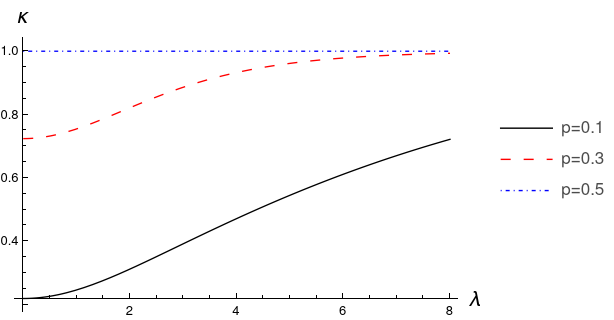
\includegraphics[width=0.6\linewidth]{maxent/figures/ContractionFactorSWAP_2D_lambda0to8.png}
  \caption{Factor de compresión $\kappa_{1}$ como función de $\lambda$, para diferentes valores de $p$.}
  \label{fig:SWAPFactor2D}
\end{figure}

Como el factor de compresión depende de $\lambda$, la dinámica no es lineal. Las operaciones cuánticas de un qubit se traducen como aplicaciones afines en la esfera de Bloch. Si quisiéramos ver el proceso asociado al \textsc{SWAP} subyacente como una transformación de la forma
\begin{equation*}
  \vec{r}\rightarrow M\vec{r}+\vec{c}
\end{equation*}
en la que $\vec{c}=0$, y $M=OS$ con $O=\Id$ y $S=\kappa_{1}(\vec{r})\Id$, de tal forma que
\begin{equation*}
  \vec{r}\rightarrow \kappa_{1}(\vec{r})\vec{r}
\end{equation*}
nos daríamos cuenta que la transformación no es afín, y por esto, el proceso no puede ser descrito a través del formalismo de las operaciones cuánticas (no tiene representación en operadores de Kraus) \cite{Chuang}.
  \begin{figure}[h!]
    \centering
    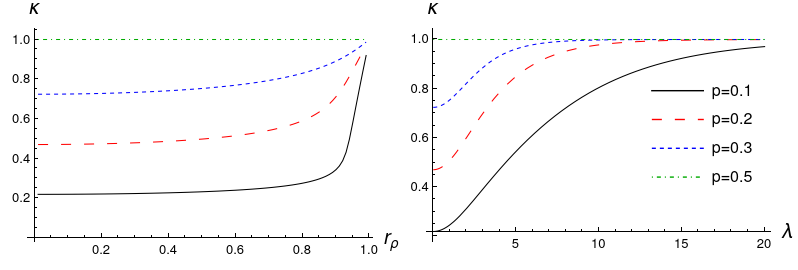
\includegraphics[width=0.9\linewidth]{maxent/figures/ContractionFactorSWAP_2D_both.png}
    \caption{Factor de compresión $\kappa_{1}$ como función de $r_{\rho}$ (der.) y como función de $\lambda$ (izq.), para diferentes valores de $p$.}
    \label{fig:SWAPFactor2Drl}
  \end{figure}
\subsubsection{Caso $p=\frac{1}{2}$}

Aunque es posible repetir todas las cuentas desde la contrucción del estado de máxima entropía, haciendo $p=\frac{1}{2}$, basta con ver que el factor (\eqref{eq:SWAPFactor}) es $1$ en dicho caso. Así, todos los estado gruesos son puntos fijos bajo una evolución subyacente SWAP con aplicación de grano grueso con parámetro $p=\frac{1}{2}$.

\subsection{Extensión a $t$}
Siendo \textsc{SWAP} un operador unitario, anteriormente se denotó el estado inicial y final como $\varrho(0)$ y $\varrho(1)$, de acuerdo a lo establecido en la ecuación (\ref{eq:TimeDepenenceUnitary}). Para extender los resultados a un tiempo arbitrario en el intervalo $[0,1]$, es necesaria una expresión analítica del operador. El operador SWAP deja intactos a los estados $\ket{00}$ y $\ket{11}$, e intercambia $\ket{01}$ con $\ket{1,0}$. De esto, el operador también dejará invariantes (hasta un factor) a los estados $\ket{+_{2}}=\frac{\ket{01}+\ket{10}}{\sqrt{2}}$ y $\ket{-_{2}}\frac{\ket{01}-\ket{10}}{\sqrt{2}}$. Dados estos eigenestados (y eigenvalores), la descomposición espectral del operador es
\begin{equation}\label{eq:SWAPSpectral}
S=P(\dyad{00}+\dyad{11}+\dyad{+_{2}}-\dyad{-_{2}})P^{\dag}.
\end{equation}
donde $P$ es la matriz formada por los eigenestados del operador. Potenciando se halla que
\begin{align}\label{eq:SWAPPower}
S^{t}&=P(\dyad{00}+\dyad{11}+\dyad{+_{2}}+(-)^{t}\dyad{-_{2}})P^{\dag}\\
&=P(\dyad{00}+\dyad{11}+\dyad{+_{2}}+e^{i \pi t}\dyad{-_{2}})P^{\dag}
\end{align}
La forma matricial del operador \textsc{SWAP} a un tiempo $t$ es
\begin{equation}
S^{t}=\begin{pmatrix}
 1 & 0 & 0 & 0 \\
 0 & \frac{1}{2}(1+e^{i \pi t}) & \frac{1}{2} (1-e^{i \pi t}) & 0 \\
 0 & \frac{1}{2}(1-e^{i \pi t}) & \frac{1}{2}(1+e^{i \pi t}) & 0 \\
 0 & 0 & 0 & 1
\end{pmatrix}=\begin{pmatrix}
  1 & 0 & 0 & 0 \\
  0 & e^{i\frac{t\pi}{2}}\cos{\frac{t\pi}{2}} & -ie^{i\frac{t\pi}{2}}\sin{\frac{t\pi}{2}} & 0 \\
  0 & -ie^{i\frac{t\pi}{2}}\sin{\frac{t\pi}{2}} & e^{i\frac{t\pi}{2}}\cos{\frac{t\pi}{2}}  & 0 \\
  0 & 0 & 0 & 1
 \end{pmatrix}
\end{equation}
Con ayuda de Mathematica pude aplicar este operador para obtener que
\begin{equation}
  \rho(t)=\frac{1}{2}\{\Id+(\hat{r_{\rho}}\cdot\vec{\sigma})[((1-p)\cos^{2}{\frac{\pi t}{2}}+p\sin^{2}{\frac{\pi t}{2}})\tanh{p\lambda}+(p\cos^{2}{\frac{\pi t}{2}}+(1-p)\sin^{2}{\frac{\pi t}{2}})\tanh{(1-p)\lambda}]\}.
\end{equation}
De esto, el factor de compresión dependiente del tiempo es
\begin{equation}\label{eq:SWAPFactort}
  \kappa_{t}^{\rho}=\frac{(p\cos^{2}{\frac{\pi t}{2}}+(1-p)\sin^{2}{\frac{\pi t}{2}})\tanh{\lambda p}+((1-p)\cos^{2}{\frac{\pi t}{2}}+p\sin^{2}{\frac{\pi t}{2}})\tanh{\lambda (1-p)}}{
    p\tanh{\lambda p}+(1-p)\tanh{\lambda (1-p)}}
\end{equation}

\begin{figure}[h!]
  \centering
  \begin{subfigure}{0.32\textwidth}
    \centering
    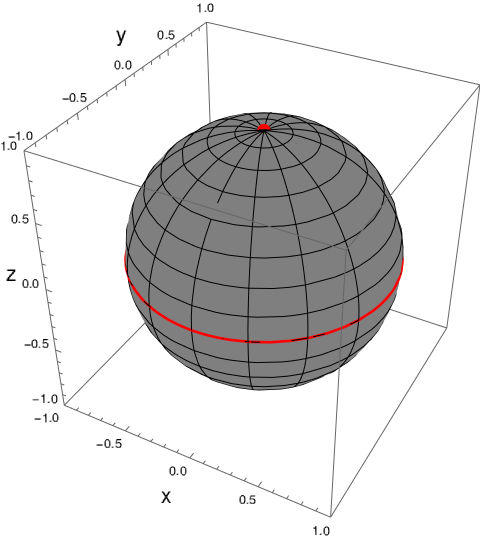
\includegraphics[width=0.9\linewidth]{maxent/figures/sphere_swapcontraction_t=0.0_z=0.9_p=0.9.png}
    \caption{$t=0$}
  \end{subfigure}%
  \begin{subfigure}{0.32\textwidth}
    \centering
    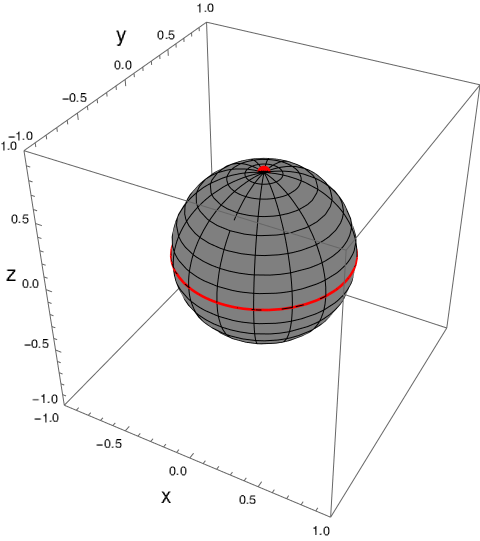
\includegraphics[width=0.9\linewidth]{maxent/figures/sphere_swapcontraction_t=0.5_z=0.9_p=0.9.png}
    \caption{$t=0.5$}
  \end{subfigure}
  \begin{subfigure}{0.32\textwidth}
    \centering
    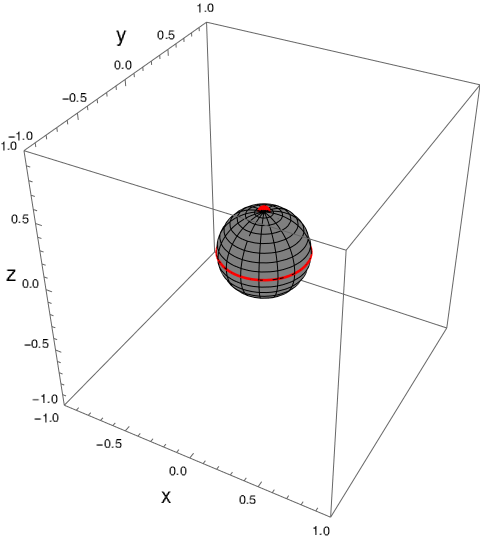
\includegraphics[width=0.9\linewidth]{maxent/figures/sphere_swapcontraction_t=1.0_z=0.9_p=0.9.png}
    \caption{$t=1$}
  \end{subfigure}
  \caption{Efecto de la evolución subyacente si $r_{z}=0.9$, $p=0.9$. La dramática contracción se asocia a una pérdida casi total de información.}
  \label{fig:SWAPFactorSequence}
  \end{figure}
En términos del valor esperado del observable $\sigma_{z}$, la evolución del estado se da como
\begin{equation}
  \expval{\sigma_{z}(t)}=\kappa_{t}^{\rho}\expval{\sigma_{z}(0)}
\end{equation}
que puede escribirse, también, como las probabilidades de que $\rho(t)$ se halle en el estado $\ket{0}$ o $\ket{1}$
 \begin{align}
  \bra{0}\rho(t)\ket{0}=\frac{1}{2}(1+\kappa_{t}^{\rho}\expval{\sigma_{z}(0)}) && \bra{1}\rho(t)\ket{1}=\frac{1}{2}(1-\kappa_{t}^{\rho}\expval{\sigma_{z}(0)}
 \end{align}
 donde la dependencia temporal está completamente contenida dentro del factor $\kappa_{t}^{\rho}$. 
\newpage